\section{抽象单纯复形}
\sourcepage{16--17}
实际处理具体多面体时，通过列出一族单形并取其并来指定多面体 $X$，并不是很方便。这样做很快就会陷入解析几何的细节：要指定所有单形，并确保它们仅在应当相交之处相交，是一件繁琐的事。通过“抽象单纯复形”来指定 $X$ 要容易得多。下面介绍这个概念。

\entry{定义}{1.4.1}\textbf{抽象单纯复形}（abstract simplicial complex）是一族有限非空集合 $\mathcal S$，满足：若 $A\in\mathcal S$，则 $A$ 的每个非空子集也属于 $\mathcal S$。

$\mathcal S$ 的元素 $A$ 称为 $\mathcal S$ 的一个\textbf{单形}，其维数等于其元素个数减 $1$。$A$ 的每个非空子集称为 $A$ 的一个面。$\mathcal S$ 的维数是其中单形维数的最大值；若不存在这样的最大值，则其维数为无限。$\mathcal S$ 的\textbf{顶点集} $V$ 是 $\mathcal S$ 中所有单点元素的并；我们不区分顶点 $v\in V$ 与 $0$ 维单形 $\{v\}\in\mathcal S$。$\mathcal S$ 的一个本身构成复形的子族，称为 $\mathcal S$ 的子复形。

若存在从抽象复形 $\mathcal S$ 的顶点集到抽象复形 $\mathcal T$ 的顶点集的双射 $f$，使得
\[
\{a_0,a_1,\ldots,a_n\}\in\mathcal S
\quad\Longleftrightarrow\quad
\{f(a_0),f(a_1),\ldots,f(a_n)\}\in\mathcal T,
\]
则称 $\mathcal S$ 与 $\mathcal T$ \textbf{同构}。

\entry{定义}{1.4.2}设 $K$ 为单纯复形，$V$ 为其顶点集。令 $\mathcal K$ 为 $V$ 中所有满足以下条件的子集 $\{a_0,a_1,\ldots,a_n\}$ 构成的族：顶点 $a_0,a_1,\ldots,a_n$ 张成 $K$ 的一个单形。族 $\mathcal K$ 称为 $K$ 的\textbf{顶点模式}（vertex scheme）。

族 $\mathcal K$ 是抽象单纯复形的一个特例。事实上，它是关键的例子，下面的定理说明了这一点。

\entry{定理}{1.4.3}
\begin{enumerate}[label=(\alph*)]
\item 每个抽象复形 $\mathcal S$ 都同构于某个单纯复形 $K$ 的顶点模式。
\item 两个单纯复形线性同构，当且仅当它们的顶点模式作为抽象单纯复形同构。
\end{enumerate}
\noindent\textbf{证明：}(b) 立即由引理 1.3.18 得到。为证明 (a)，作如下构造。给定指标集 $J$，令 $\Delta^J$ 为 $E^J$ 中由标准基 $\{\epsilon_\alpha\}_{\alpha\in J}$ 的有限子集张成的所有单形构成的族。容易看出，$\Delta^J$ 是单纯复形。如果 $\sigma,\tau$ 是其中两个单形，则它们的顶点集合在一起仍几何独立，并张成 $\Delta^J$ 的一个单形。若 $J$ 为无限集，则 $\Delta^J$ 是一个无限维单形。\translatornote{此处“无限维单形”沿用原文的称呼；严格地说，$\Delta^J$ 是由所有有限维面构成的复形，而非前面定义中的某个有限维单形。}

现设 $\mathcal S$ 的顶点集为 $V$。选取足够大的指标集 $J$，使存在单射 $f:V\to\{\epsilon_\alpha\}_{\alpha\in J}$，例如可取 $J=V$。如下指定 $\Delta^J$ 的一个子复形 $K$：对于每个［抽象］单形 $\{a_0,\ldots,a_n\}\in\mathcal S$，由 $f(a_0),\ldots,f(a_n)$ 张成的［几何］单形属于 $K$。显然，$K$ 是单纯复形，而且 $\mathcal S$ 同构于 $K$ 的顶点模式；$f$ 就是两个顶点集之间所需的对应。\hfill$\square$

\entry{定义}{1.4.4}若抽象单纯复形 $\mathcal S$ 同构于单纯复形 $K$ 的顶点模式，则称 $K$ 为 $\mathcal S$ 的一个\textbf{几何实现}（geometric realization）。在相差一个线性同构的意义下，几何实现唯一确定。

下面举例说明，如何利用抽象复形指定具体的单纯复形。

\entry{例}{1.4.5}假定要指定一个单纯复形 $K$，使其底空间同胚于圆柱面 $S^1\times I$，其中 $I$ 表示闭单位区间 $[0,1]$。一种方法是画出图 1.4.1，它把 $K$ 指定为由六个 $2$ 维单形及其各个面组成的族。
\begin{center}
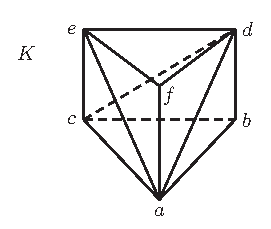
\includegraphics[width=46mm]{figures/1-4-1.pdf}\\图 1.4.1
\end{center}
\sourcepage{18}
表示同一复形 $K$ 的另一种方法是画出图 1.4.2。该图包含两部分：第一，一个底空间为矩形的复形 $L$；第二，对 $L$ 的顶点作出的特定标记，其中某些顶点使用相同的标记。我们把这张图视为如下抽象复形 $\mathcal S$ 的简写：顶点集为字母 $a,b,c,d,e,f$，其单形为
\[
\{a,f,d\},\ \{a,b,d\},\ \{b,c,d\},\ \{c,d,e\},\ \{a,c,e\},\ \{a,e,f\}
\]
以及这些集合的所有非空子集。当然，这个抽象复形同构于先前图中复形 $K$ 的顶点模式，因而在相差线性同构的意义下，它精确指定了同一个复形。也就是说，图 1.4.1 中的 $K$ 是 $\mathcal S$ 的一个几何实现。
\begin{center}
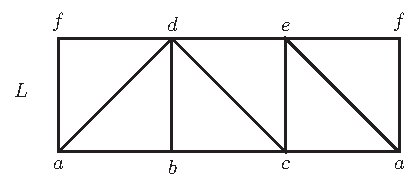
\includegraphics[width=77mm]{figures/1-4-2.pdf}\\图 1.4.2
\end{center}
令 $f:L^{(0)}\to K^{(0)}$ 将 $L$ 的每个顶点映到 $K$ 中具有相同标记的对应顶点。则 $f$ 扩张为单纯映射 $g:|L|\to|K|$。由于这些空间是紧致 Hausdorff 空间，$g$ 是商映射，也就是“粘合映射”。它把 $|L|$ 的右边与左边作线性等同。这正是用一张矩形纸片做成圆柱面的通常方法：把纸片弯过来，将右边粘到左边！

\entry{例}{1.4.6}现在从复形 $L$ 及其顶点的一种标记方式出发。例如，对同一个 $L$ 作另一种顶点标记，如图 1.4.3。与前面一样，这张图指定了某个抽象复形 $\mathcal S$，可以逐一列出其单形。设 $K$ 为 $\mathcal S$ 的几何实现。$K$ 的顶点仍对应于字母 $a,b,\ldots,f$。考虑线性单纯映射 $g:|L|\to|K|$，把 $L$ 的每个顶点映到 $K$ 中具有相同标记的顶点。$g$ 仍是商映射；此时它把 $|L|$ 的左边与右边作线性等同，但要扭转一下。空间 $|K|$ 就是所谓的 \textbf{Möbius 带}。它可以在 $\R^3$ 中画成图 1.4.3 所示的熟悉形状。
\begin{center}
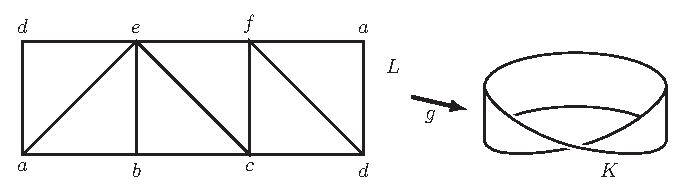
\includegraphics[width=113mm]{figures/1-4-3.pdf}\\图 1.4.3
\end{center}

\sourcepage{19--20}
\entry{例}{1.4.7}\textbf{环面}通常定义为对矩形作图 1.4.4 所示等同而得到的商空间。若要构造底空间同胚于环面的复形，就可以使用图 1.4.5。可以验证，从 $L$ 到此图的几何实现的商映射，恰好完成了构造环面所需要的各项等同。
\begin{center}
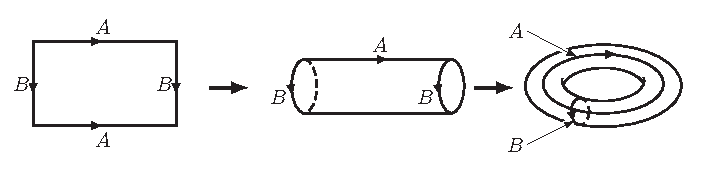
\includegraphics[width=114mm]{figures/1-4-4.pdf}\\图 1.4.4
\medskip

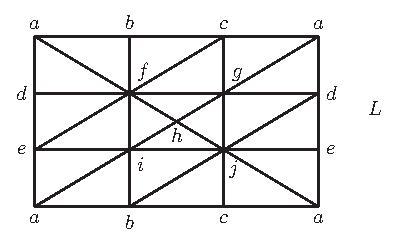
\includegraphics[width=68mm]{figures/1-4-5.pdf}\\图 1.4.5
\end{center}
\entry{例}{1.4.8}一般地，需要小心，确保商映射 $g$ 不会进行超出预期的等同。例如，你可能以为图 1.4.6 确定了环面，其实并非如此。仔细观察该图就会发现，这时的商映射除了把对边粘合，还作了额外的等同。
\begin{center}
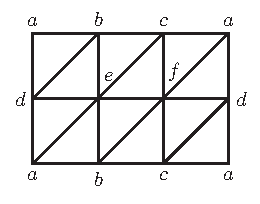
\includegraphics[width=48mm]{figures/1-4-6.pdf}\\图 1.4.6
\end{center}
\entry{例}{1.4.9}图 1.4.7 指定了一个抽象复形，其底空间称为 \textbf{Klein 瓶}。它是将矩形的各边按照图 1.4.8 所示方式粘合得到的商空间。所得空间不能嵌入 $\R^3$，但可以允许它“穿过自身”，从而在 $\R^3$ 中画出示意图。
\begin{center}
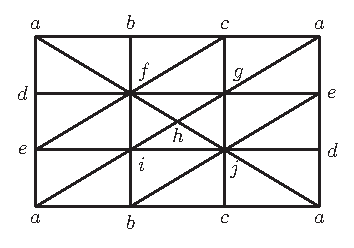
\includegraphics[width=65mm]{figures/1-4-7.pdf}\\图 1.4.7
\medskip

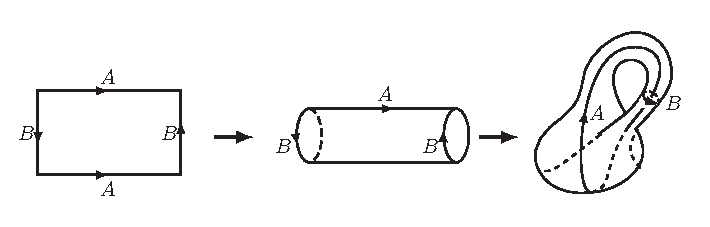
\includegraphics[width=114mm]{figures/1-4-8.pdf}\\图 1.4.8
\end{center}
\entry{例}{1.4.10}\textbf{射影平面} $P^2$ 定义为将二维球面 $S^2$ 中每个点 $x$ 与 $-x$ 等同而得到的空间。习题 2(b) 要求证明：图 1.4.9 确定了一个底空间同胚于 $P^2$ 的复形。\translatornote{原文引用“习题 2(b)”，但本节实际对应的是习题 1(b)。}
\begin{center}
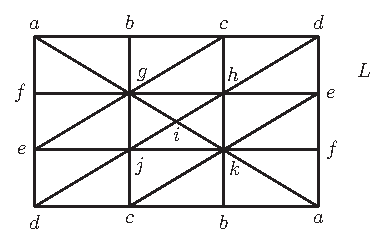
\includegraphics[width=68mm]{figures/1-4-9.pdf}\\图 1.4.9
\end{center}
现在更仔细地说明前面各例所用的过程。给定有限复形 $L$，对其顶点作\textbf{标记}，就是给出从 $L$ 的顶点集到某个集合的满射 $f$，该集合称为\textbf{标记集}。相应的抽象复形 $\mathcal S$ 以这些标记为顶点，其单形为所有形如 $\{f(v_0),\ldots,f(v_n)\}$ 的集合，其中 $v_0,\ldots,v_n$ 张成 $L$ 的一个单形。设 $K$ 为 $\mathcal S$ 的几何实现。由 $f$ 得到的从 $L^{(0)}$ 到 $K^{(0)}$ 的顶点满射扩张为满的单纯映射 $g:|L|\to|K|$。称 $K$ 为\textbf{由带标记复形导出的复形}，称 $g$ 为\textbf{相应的粘合映射}。

由于 $|L|$ 紧致而 $|K|$ 是 Hausdorff 空间，$g$ 把闭集映为闭集，因此 $g$ 是闭商映射。当然，一般地，$g$ 可能把 $L$ 的某个单形映到 $K$ 的一个较低维单形上。例如，$g$ 可能把整个 $L$ 压缩为一个点。我们更关心不会发生这种情况的情形，特别是与前面各例类似的情况。下面的引理给出一般粘合映射 $g$ 具有这些例子中行为的条件。首先需要一个定义。

\sourcepage{21--22}
\entry{定义}{1.4.11}设 $L$ 为复形。如果 $L$ 中每个所有顶点都属于子复形 $L_0$ 的单形，本身也属于 $L_0$，就称 $L_0$ 为 $L$ 的\textbf{满子复形}（full subcomplex）。

例如，图 1.4.5 中矩形 $L$ 的边界是 $L$ 的满子复形，但图 1.4.6 中矩形的边界则不是。

\entry{引理}{1.4.12}设 $L$ 为复形，$f$ 是其顶点的一种标记，$g:|L|\to|K|$ 为相应的粘合映射，$L_0$ 为 $L$ 的满子复形。假设只要 $L$ 的顶点 $v,w$ 具有相同标记，就有：
\begin{enumerate}[label=(\arabic*)]
\item $v,w$ 属于 $L_0$。
\item $\overline{\operatorname{St}v}$ 与 $\overline{\operatorname{St}w}$ 不相交。
\end{enumerate}
则对于所有 $\sigma\in L$，有 $\dim g(\sigma)=\dim\sigma$。此外，若 $g(\sigma_1)=g(\sigma_2)$，则 $\sigma_1,\sigma_2$ 必须是属于 $L_0$ 的不相交单形。\translatornote{此处按原文译出；条件中的顶点应理解为两个不同顶点，结论中的 $\sigma_1,\sigma_2$ 也应理解为两个不同单形，否则取两者相同便不成立。}

证明很容易，留作习题。通常应用这个引理时，$|L|$ 是平面或 $\R^N$ 中的某个多面体区域，$|L_0|$ 是该区域的边界。

\subsection*{习题}
\begin{enumerate}
\item \begin{enumerate}[label=(\alph*)]
\item 证明，$P^2$ 同胚于从 $B^2$ 出发，将每个 $x\in S^1$ 与 $-x$ 等同所得到的空间。
\item 证明图 1.4.9 中的带标记复形 $L$ 确定了一个底空间同胚于 $P^2$ 的复形 $K$。
\item 描述图 1.4.10 中带标记复形所确定的空间。
\end{enumerate}
\begin{center}
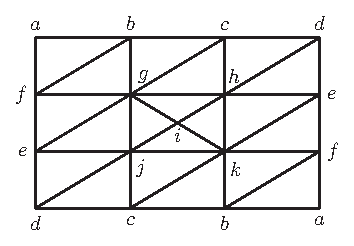
\includegraphics[width=65mm]{figures/1-4-10.pdf}\\图 1.4.10
\end{center}
\item 描述图 1.4.11--1.4.14 中各带标记复形所确定的空间。
\begin{center}
\begin{minipage}{.45\textwidth}\centering
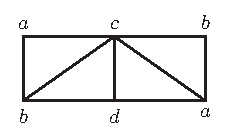
\includegraphics[width=47mm]{figures/1-4-11.pdf}\\图 1.4.11
\end{minipage}\hfill
\begin{minipage}{.45\textwidth}\centering
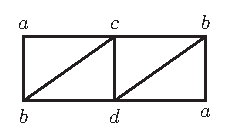
\includegraphics[width=47mm]{figures/1-4-12.pdf}\\图 1.4.12
\end{minipage}
\medskip

\begin{minipage}{.43\textwidth}\centering
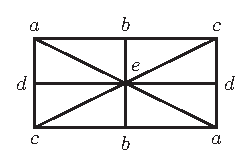
\includegraphics[width=45mm]{figures/1-4-13.pdf}\\图 1.4.13
\end{minipage}\hfill
\begin{minipage}{.53\textwidth}\centering
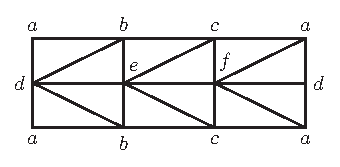
\includegraphics[width=64mm]{figures/1-4-14.pdf}\\图 1.4.14
\end{minipage}
\end{center}
\item 证明引理 1.4.12。
\item 设 $S$ 为带偏序关系 $\leq$ 的集合。组合数学中的一种标准方法是，将抽象复形 $\mathcal S$ 与 $S$ 联系起来：$\mathcal S$ 的顶点是 $S$ 的元素，单形是 $S$ 的有限全序子集。假设 $\{a_1,a_2,\ldots,a_8\}$ 上的偏序由下列关系生成：
\[
\begin{aligned}
a_1&\leq a_3\leq a_7\leq a_8;& a_1&\leq a_5\leq a_7;\\
a_2&\leq a_6\leq a_8;& a_2&\leq a_5.
\end{aligned}
\]
描述 $\mathcal S$ 的一个几何实现。
\end{enumerate}
